\chapter{Analysis of Parasite Clearance Times}\label{ch:analysis}
The derived PC90 values using the log-linear interpolation method are shown in Table \ref{derivedPC90}.
\begin{table}[h]
\centering
\caption{Derived PC90 values in hours}\label{derivedPC90}
\begin{tabular}{|cc|c|c|}
\hline
&&\multicolumn{2}{c|}{Treatment}\\
&&alone&combined\\\hline
\multirow{2}{*}{Centre 1}&Male&$\begin{array}{c}3.85,\ 27.32,\ 36.30,\  8.84,\\4.35,\  1.53,\ 30.01,\  4.83\end{array}$&$\begin{array}{c}9.47,\  5.05,\  8.10,\\22.77,\  9.40,\  7.73\end{array}$\\\cline{2-4}
&Female&$\begin{array}{c}19.76,\ 22.45,\\21.75,\ 46.52\end{array}$&$\begin{array}{c}3.65,\ 8.40 ,\ 9.69,\\0.85,\ 9.04,\ 9.38\end{array}$\\\hline
\multirow{2}{*}{Centre 2}&Male&$\begin{array}{c}4.82,\ 2.21,\\11.59,\ 28.09\end{array}$&$\begin{array}{c}17.15,\ 9.51,\\14.68,\ 8.08\end{array}$\\\cline{2-4}
&Female&$\begin{array}{c}21.97,\ 2.49,\ 25.08,\ 31.63,\\5.00,\ 21.64,\ 24.42\end{array}$&$\begin{array}{c}14.77,\  8.75,\\5.84,\ 6.23\end{array}$\\\hline
\end{tabular}
\end{table}
Summary statistics are shown in Table \ref{summaryPC90}.
\begin{table}
\centering
\caption{Summary statistics for PC90 in hours}\label{summaryPC90}
\begin{tabular}{|l|ccc|ccc|}
\hline
&\multicolumn{6}{c|}{Treatment}\\
&\multicolumn{3}{c|}{alone}&\multicolumn{3}{c|}{combined}\\
&mean&median&sd&mean&median&sd\\
\hline
Centre 1	& 19.0 & 20.8 & 14.5 & 8.6  &  8.7  &  5.2 \\
Centre 2	& 16.3  & 21.6 &  11.2 & 10.6  &  9.1  &  4.3 \\
\hline
Male		& 13.6  &  6.8 & 12.9 & 11.2  &  9.4 &   5.4 \\
Female	& 22.1  & 22.0 &  11.8 & 7.7  &  8.6  &  3.8  \\
\hline
All		& 17.7  & 21.6 &  12.8 & 9.4  &  8.9  &  4.9  \\
\hline 
\end{tabular}
\end{table}

It can be seen that PC90 is generally shorter for subjects on the single drug (``alone'') treatment than those on the combined drug treatment across both centres. However, male patients have a higher median PC90 on the combined treatment. Standard deviations are notably higher for the single treatment. There do not seem to be any clear differences between centres. Females have longer PC90 times than males on the alone treatment with the opposite trend on the combined treatment.

\section{Graphical comparison}
The PC90 data from Table \ref{derivedPC90} are plotted by factors centre, sex and treatment in Figure \ref{pc90boxes}, summarized in two ways. Firstly, by the median and upper and lower quartiles. Secondly, the mean is shown with 95\% confidence intervals from the $t$ distribution defined by the standard error of the data%\footnote{The $t$ distribution confidence intervals are calculated using the \texttt{smean.cl.normal} \emph{R} functions from the Hmisc library \cite{Hmisc}}
. These confidence intervals for the mean are relevant for parametric tests based on the normal distribution such as ANOVA and give an indication of differences that may be significant.
\begin{figure}[h]
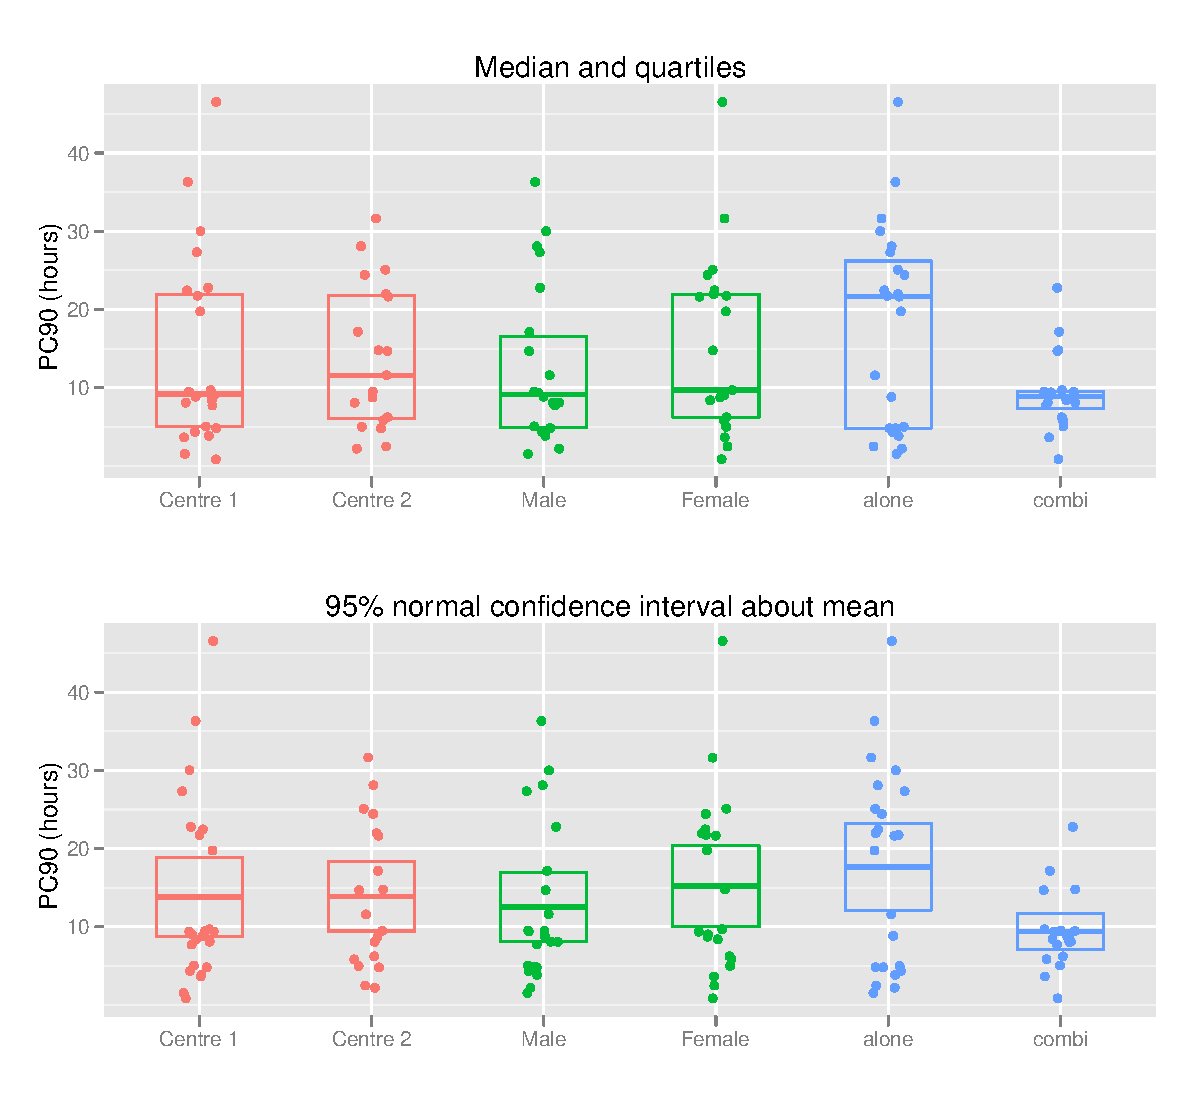
\includegraphics[width=150mm]{pc90boxes.eps} 
\caption{Comparison of PC90 by experimental factors with box plots showing medians and quartiles (top) and means with $t$ distribution 95\% confidence intervals (bottom)}
\label{pc90boxes}
\end{figure}

It can be seen in Figure \ref{pc90boxes} that there doesn't seem to be any notable difference in clearance times between centres. Female subjects seem to have a larger variance in clearance times and perhaps a slightly longer clearance time on average. The difference in clearance times due to the treatment chosen seems to have the largest influence with a larger spread in clearance times for subjects on the ``alone'' single-drug treatment with a potentially significant decrease in mean clearance time for the subjects on the combined-drug treatment.

An additional observation is that the distributions seem bimodal in the cases of the centre 1, female and alone treatment subjects. Looking at the plots of PC90 derivation in the previous chapter (Figures \ref{pc90-agree} to \ref{pc90-nofit}), it is not clear why this is. There does not seem to be an indication that this would arise due to the fitting method and hence it is likely to be a real feature of the clearance times.

In Figure \ref{pc90interaction} the data is split by pairs of factors in each plot to look for interaction effects between the factors. Again, the mean and 95\% confidence intervals for the mean are shown.
\begin{figure}[h]
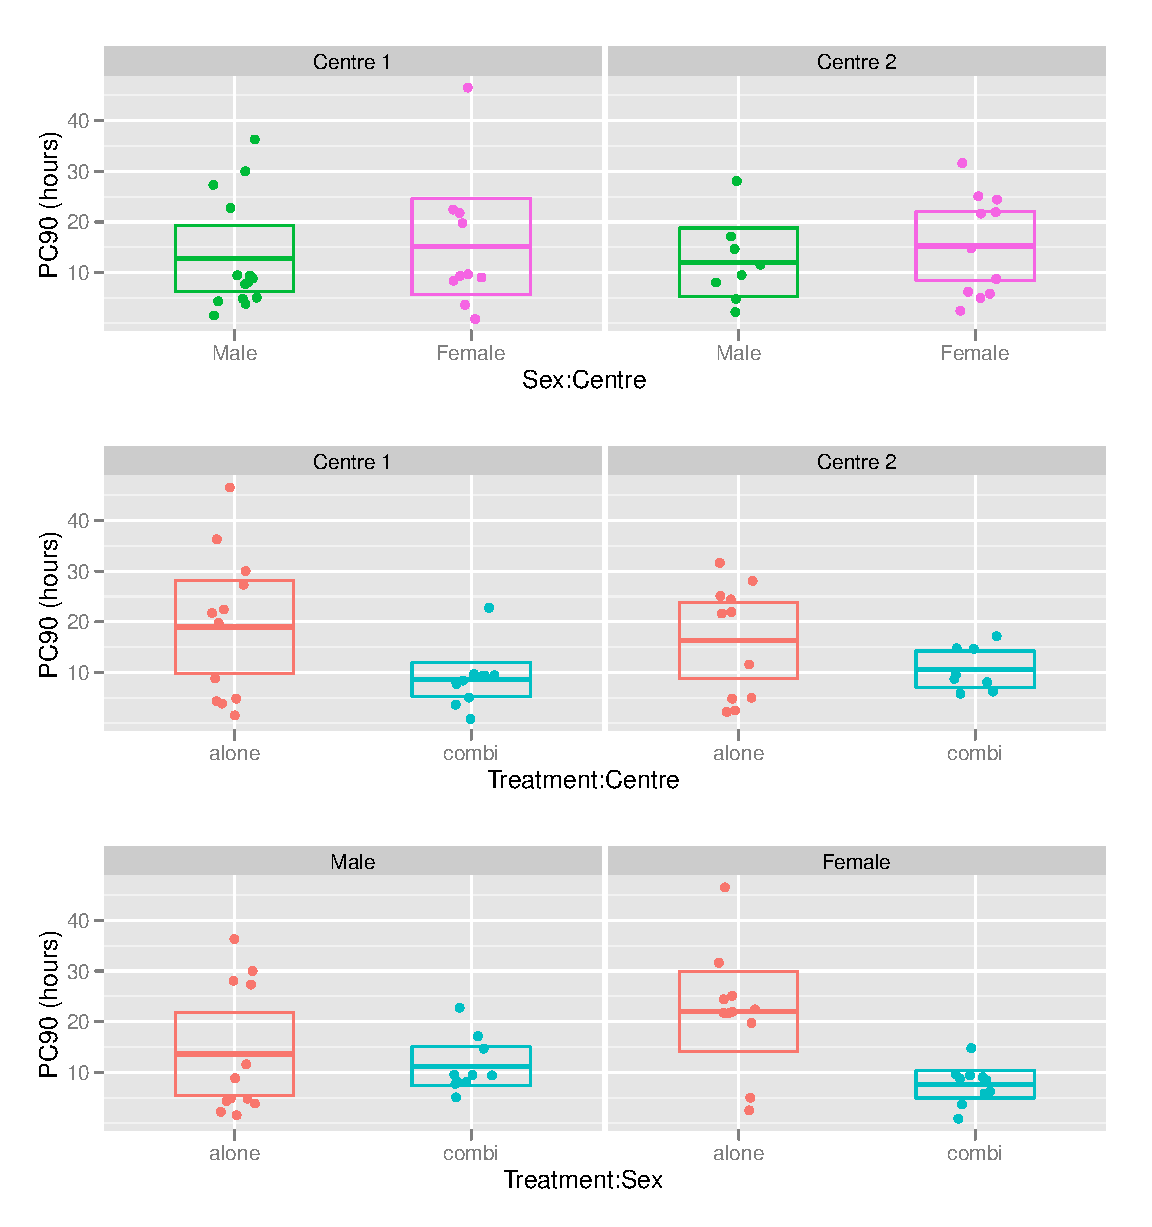
\includegraphics[width=150mm]{pc90interaction.eps} 
\caption{PC90 with 95\% confidence intervals for the means plotted by pairs of factors to look for two-way interactions}
\label{pc90interaction}
\end{figure}
It can be seen that there doesn't seem to be any interaction between sex and centre or treatment and centre i.e. the left and right panels of the top two plots look essentially the same. However, it appears that the combined treatment only decreases the mean clearance time for female subjects.
\clearpage
\section{ANOVA modelling by experimental factors}
3-way ANOVA with all interactions was performed on the PC90 data in Table \ref{derivedPC90}. The fitted model is
\begin{eqnarray}
&\mathrm{PC}90_{ijkl}=\mu+C_i+S_j+T_k+(CS)_{ij}+(CT)_{ik}+(ST)_{jk}+(CST)_{ijk}+\epsilon_{ijkl}&\nonumber\\
&\epsilon_{ijkl}\sim N(0,\sigma^2)&\label{full}
\end{eqnarray}
where PC$90_{ijkl}$ is the clearance time for subject $l$ in centre $i$, of sex $j$ on treatment $k$; $C_i$ is the effect of the centre, $S_j$ the effect of the sex; $T_k$ the treatment effect; $(CS)_{ij}$ the interaction effect of centre and sex and so on ($i,j,k=1,2$). Using a corner-point constraint, $\mu$ corresponds to the expected PC90 for a centre 1, male on the single-drug treatment, with all other terms in the model representing the difference from this mean.

The standardized residuals ($e/\hat{\sigma}$) obtained from fitting model \ref{full} are plotted in Figure \ref{aovloglinres}.
\begin{figure}[ht]
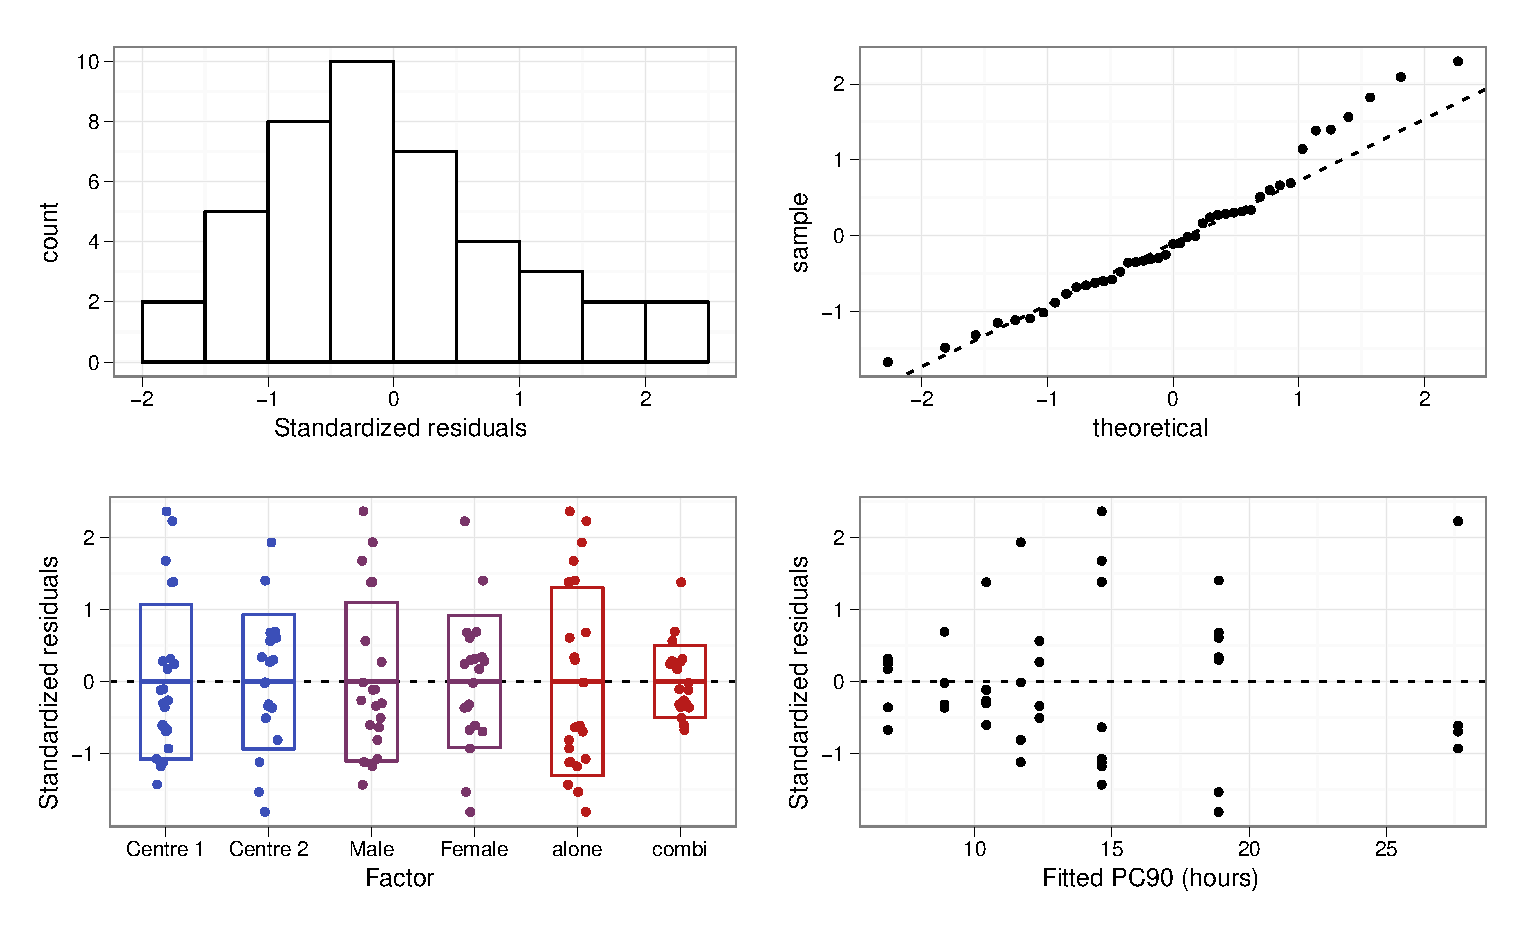
\includegraphics[width=150mm]{aovloglinres.eps} 
\caption{Residuals for 3-way ANOVA model for PC90 with all interactions}
\label{aovloglinres}
\end{figure}

It can be seen that the residuals are approximately normally distributed, but perhaps slightly right skewed. In the plot of the residuals by experimental factor (bottom-left) the standard deviation of the residuals is shown as the upper and lower edges of the rectangles. The standard deviation of standardized residuals should be approximately 1 and independent of factor. We can see that this is so for centre and sex, but there is heteroscedasticity between treatments with the residuals for the single-drug treatment showing a larger variance than for the combined-drug treatment.
%($P<0.05$ under a Breusch-Pagan test for heteroscedasticity \cite{breusch} as implemented by the \texttt{bptest} \emph{R} function \cite{lmtest}).
We can also see that the variance of the residuals increases with fitted PC90 value (bottom-right).

\subsection{Dealing with heteroscedasticity}
Least squares estimators are still unbiased under heteroscedasticity, but standard errors can be underestimated leading to incorrect inference \cite{long}. Two ways we can adapt our modelling to deal with heteroscedasticity are to transform the dependent variable and to use weighted least-squares fitting.

\subsubsection*{Transforming the dependent variable}
If we apply a square-root transformation to PC90 we obtain the residuals for the ANOVA model shown in Figure \ref{aovsqrtres}.
\begin{figure}[h]
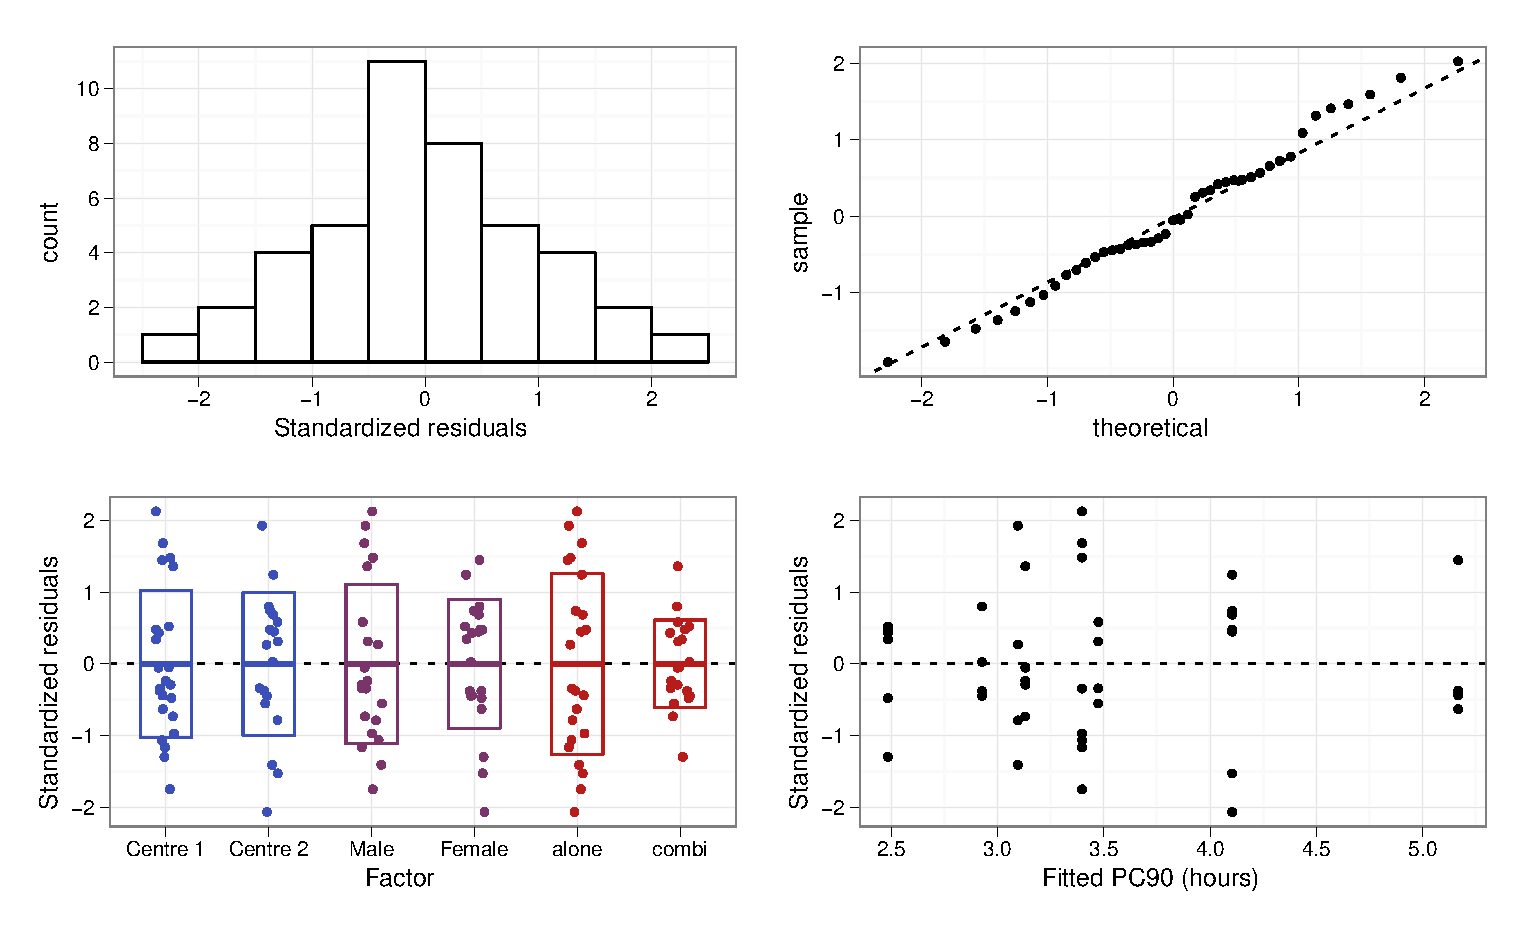
\includegraphics[width=150mm]{aovsqrtres.eps} 
\caption{Residuals after applying a square-root transformation to the dependent variable}
\label{aovsqrtres}
\end{figure}
It can be seen that this transformation reduces the correlation of the variance of the residuals with fitted PC90. Other transformations, such as logarithmic or square, did not prove as suitable as a square-root transformation. The Box-Cox method, whereby the transformation giving the highest likelihood is found, suggests transforming the dependent variable by raising it to the power 0.3 is optimal. This did not appear to give a noticeable improvement over the square-root transformation (power 0.5) in residual plots however.

It can be seen that, even after our square-root transformation, the residuals for subjects on the combined treatment have a smaller variance than for those on the single treatment. Bartlett's test for equality of variances \cite{montgomery} between the 8 ($2^{3}$) centre-sex-treatment groups gives evidence to reject the hypothesis that the variance is equal in all groups ($P<0.05$).  One common method of dealing with heteroscedastic residuals between groups is to use weighted least-squares.

\subsubsection*{Weighted least-squares}
In this case, to remedy the heteroscedasticity between treatment groups, we weight the fitting by the variance within treatment groups such that error term in model \ref{full} becomes 
\begin{equation}
\epsilon_{ijkl}\sim N(0,\sigma^2\sigma_{k}^{2})\label{wls}
\end{equation}
where $\sigma_{k=1}^{2}$ is the variance of subjects on the single treatment, $\sigma_{k=2}^{2}$ is the variance of subjects on the combined treatment and we estimate $\sigma^{2}$. This model is fitted by minimizing
\begin{equation*}
S=\sum_{ijkl} w_{k}(\mathrm{PC}90_{ijkl} - \widehat{\mathrm{PC}90_{ijk}})^{2}
\end{equation*}
where the weights $w_{k}=\sigma_{k}^{-2}$. The residuals from fitting this function using the \texttt{weights} parameter of the \emph{R} linear least-squares \texttt{lm} function are shown in Figure \ref{aovresw}.
\begin{figure}[p]
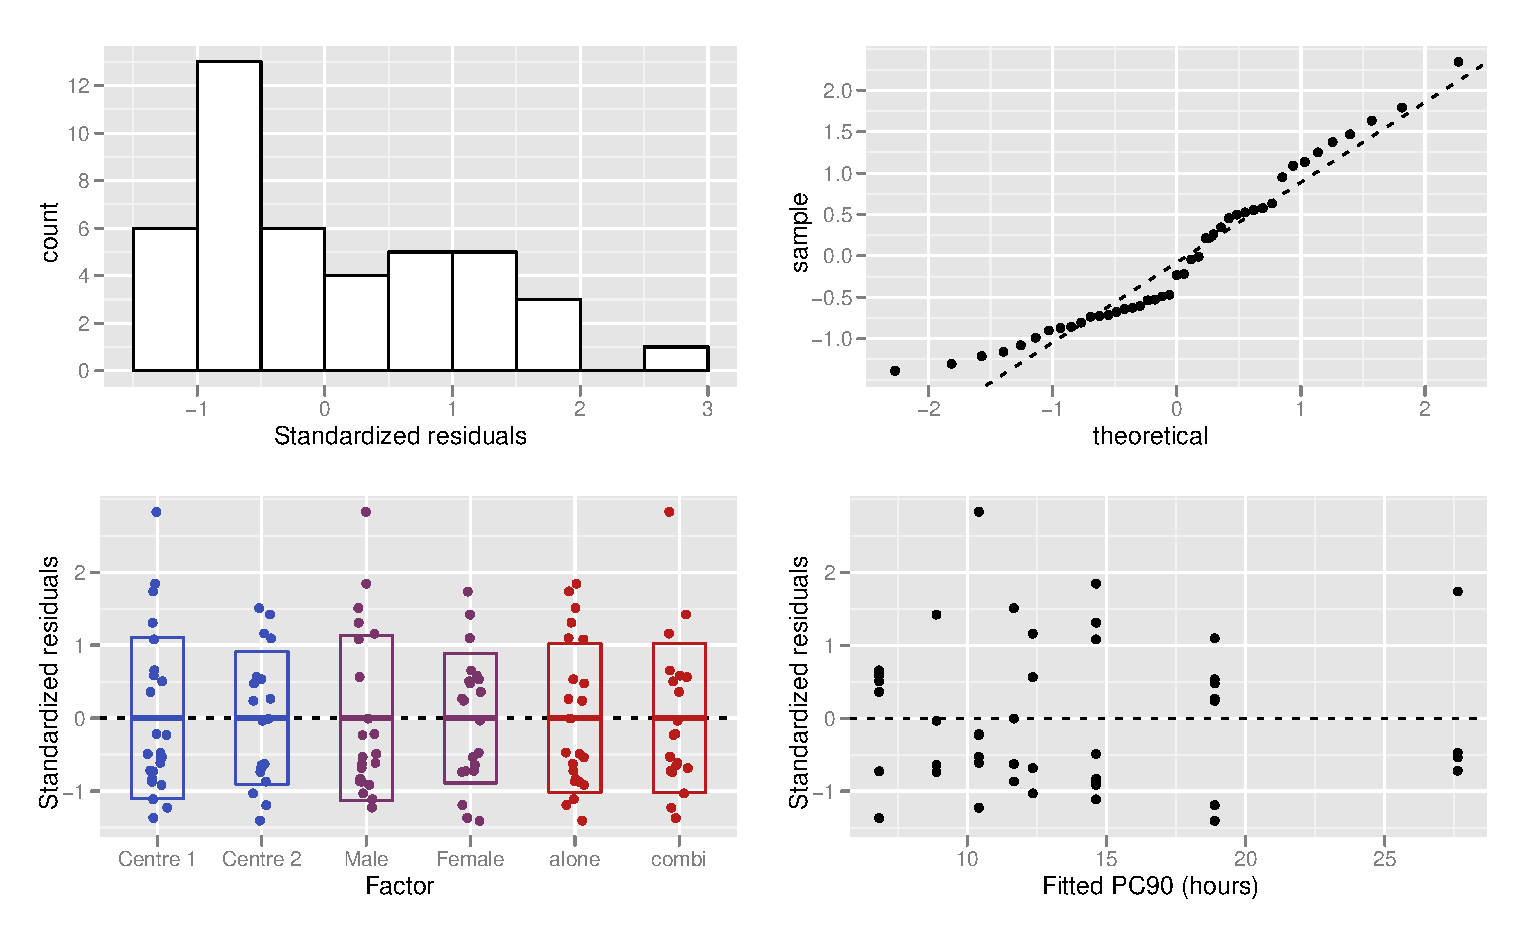
\includegraphics[width=150mm]{aovresw.eps} 
\caption{Residuals after applying weighted least squares}
\label{aovresw}
\end{figure}
The residuals now have approximately equal variance with respect to factor and fitted PC90, but they appear to be right-skewed.

If we apply the square-root transformation followed by the treatment-variance weighted least-squares fit we obtain the residuals shown in Figure \ref{aovsqrtresw}.
\begin{figure}[p]
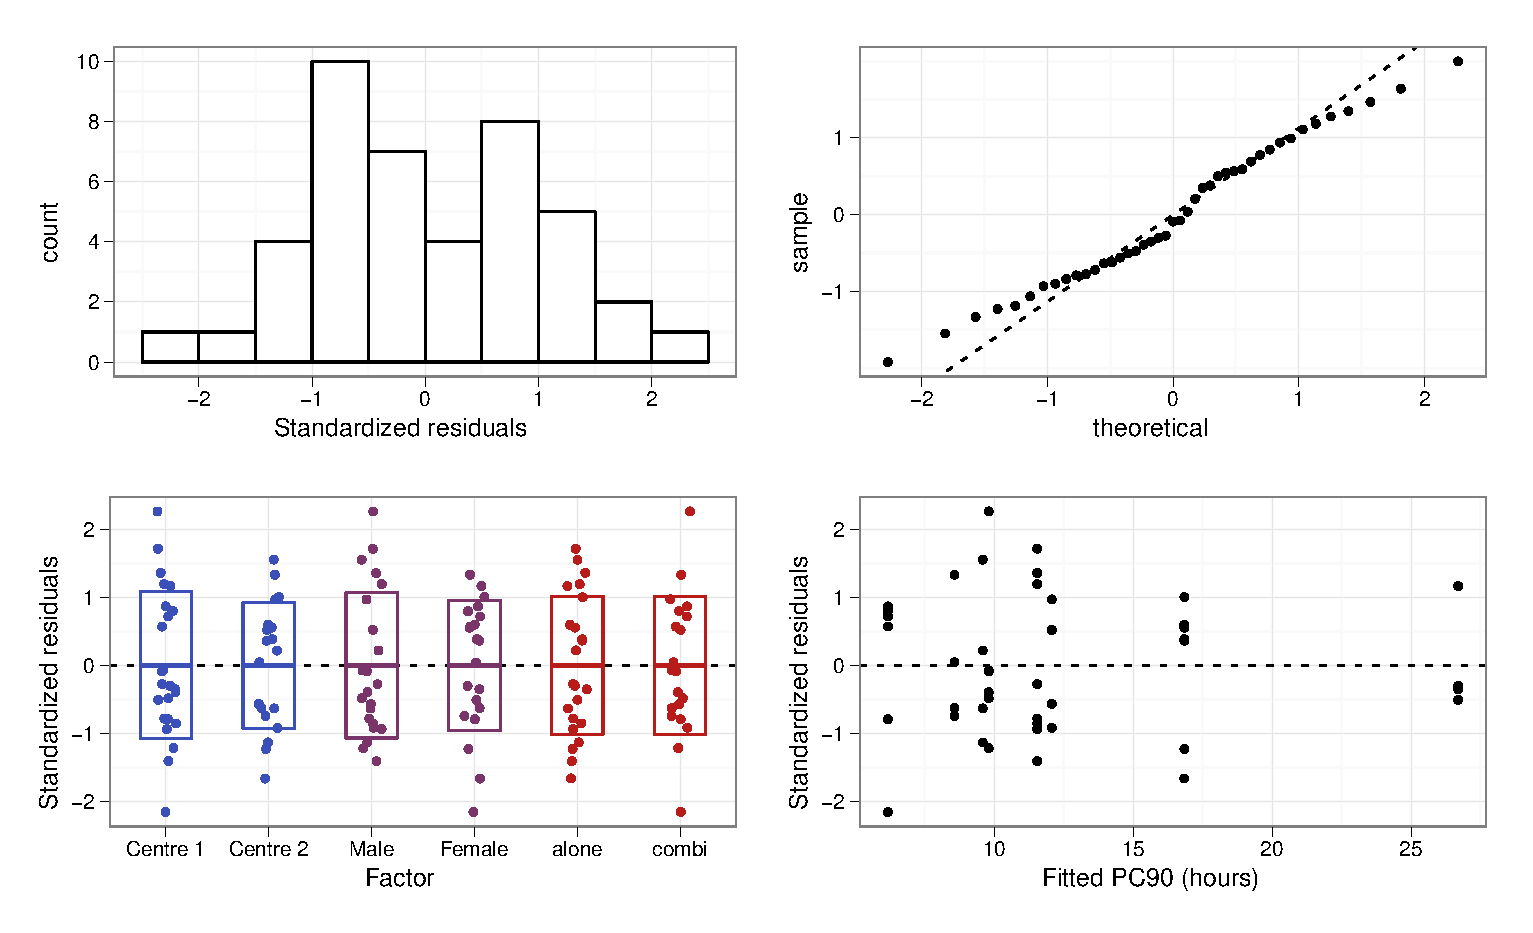
\includegraphics[width=150mm]{aovsqrtresw.eps} 
\caption{Residuals after applying square-root transformation and weighted least squares}
\label{aovsqrtresw}
\end{figure}
This seems to give a more symmetric distribution of residuals but is perhaps a bit light-tailed.
Despite this, none of the distributions of residuals show evidence of significant departures from normality by a Shapiro-Wilk test and there also now seems to be no significant difference in the variance of the residuals between experimental groups.

\subsection{Model selection}
Now that we seem to have a transformation such that the assumptions of our model are met we can start to look at hypothesis tests on the experimental factors. Table \ref{aovwt} shows the results of the ANOVA analysis for model \ref{full} using  weighted least-squares. Table \ref{aovsqrtwt} shows the results for the model using a square root transformation and weighted least-squares.
\begin{table}[h]
\centering
\caption{ANOVA table for full model fitted by weighted least-squares}\label{aovwt}
\begin{tabular}{l|rrrrrl}
Source&Sum Sq.&df&Mean Sq.&$F$&P($>F$)\\
\hline
$Centre$     &                0.631  &1& 0.631 & 0.654 &0.424&\\
$Sex$        &              0.972  &1& 0.972 & 1.01 &0.322\\
$Treatment$  &            7.85  &1& 7.85  &8.14 &0.007 &**\\
$Centre\times Sex$ &             0.001 &1&  0.001 & 0.001 &0.975&\\
$Centre\times Treatment$ &        0.511  &1& 0.511 & 0.530 &0.472&\\
$Sex\times Treatment$     &     5.21  &1& 5.21 & 5.40 &0.026 &* \\
$Centre\times Sex\times Treatment$ &   0.239 &1&  0.239 & 0.247& 0.622&\\
$Residuals$      &    33.76 &35&  0.965  &&&\\
\hline
Total&49.17&42&&&
\end{tabular}\\
\hspace{20em}*$<0.05$\quad**$<0.01$
\end{table}
\begin{table}[h]
\centering
\caption{ANOVA table for full model with square-root transformation fitted by weighted least-squares}\label{aovsqrtwt}
\begin{tabular}{l|rrrrrl}                   
Source&Sum Sq.&df&Mean Sq.&$F$&P($>F$)\\
\hline
$Centre$     &                0.834 &1&  0.834 & 0.882 & 0.354 &\\    
$Sex$        &               0.630 &1&  0.630 & 0.666 & 0.420 &\\  
$Treatment$  &            4.89 &1&  4.89 &  5.17 & 0.029& *\\
$Centre\times Sex$ &             0.003 &1& 0.003 & 0.003 & 0.956&\\
$Centre\times Treatment$ &        0.523 &1&  0.523 & 0.553 & 0.462&\\
$Sex\times Treatment$     &     5.94 &1& 5.94 & 6.28 & 0.017& *\\
$Centre\times Sex\times Treatment$ &   0.271 &1&  0.271 & 0.287 & 0.596&\\
$Residuals$      &    33.118 &35&  0.946 &&&\\
\hline
Total&46.21&42&&&
\end{tabular}\\
\hspace{20em}*$<0.05$
\end{table}

It can be seen that there is no evidence to reject the hypothesis that the centre has negligible effect on the clearance time. 
%\subsubsection*{Non-parametric check on $p$-values}
%We checked that our residuals were approximately normally distributed and homoscedastic and so our hypothesis tests and standard errors, based on these assumptions, should be accurate. However, we can perform an additional non-parametric validation by resampling methods.

%If we randomize the clearance times among the 43 patients and then refit our model and calculate the $F$ statistic for each randomization we can construct the empirical distribution of the statistic and obtain $p$-values from this. This was done using 10,000 samples and the results are shown in Table \ref{aovresamp}, where the $p$-value from the F distribution ($P_{F}$), the empirical distribution obtained by randomising ($P_{rand}$) and the empirical bootstrap distribution ($P_{boot}$), whereby instead of randomising the 43 values, we resample with replacement.
%\begin{table}[h]
%\centering
%\caption{Comparison of parametric $p$-values and $p$-values from resampling}\label{aovresamp}
%\begin{tabular}{l|rrrr|rrrrl}
%&\multicolumn{4}{c}{Weighted LSQ}&\multicolumn{4}{c}{Sqrt weighted LSQ}&\\                   
%Source&$F$&$P_{F}$&$P_{rand}$&$P_{boot}$&$F$&$P_{F}$&$P_{rand}$&$P_{boot}$&\\
%\hline
%$Centre$     						& 0.654 & 0.424 & 0.536 & 0.547     	& 0.882 & 0.354 & 0.434 & 0.437 &\\    
%$Sex$        						& 1.01   & 0.322 & 0.440 & 0.446     	& 0.666 & 0.420 & 0.498 & 0.500 &\\  
%$Treatment$ 						& 8.14   & 0.007 & 0.001 & 0.002     	& 5.17   & 0.029 & 0.012 & 0.012 &*\\
%$Centre\times Sex$ 					& 0.001 & 0.975 & 0.982 & 0.981     	& 0.003 & 0.956 & 0.962& 0.964 &\\
%$Centre\times Treatment$			& 0.530 & 0.472 & 0.322 & 0.328	& 0.553 & 0.462 & 0.381& 0.375 &\\
%$Sex\times Treatment$     			& 5.40   & 0.026 & 0.003 & 0.003	& 6.28   & 0.017 & 0.005& 0.005 &*\\
%$Centre\times Sex\times Treatment$	& 0.247 & 0.622 & 0.482 & 0.491	& 0.287 & 0.596 & 0.507& 0.516 &\\
%\hline
%\end{tabular}
%\end{table}

%It can be seen that the $p$-values obtained by the parametric and non-parametric methods are in general agreement, although the F test seems more conservative than the non-parametric tests. In all 3 cases it can be seen that there is no evidence to reject the hypothesis that the effect of the centre is negligible.

\subsubsection*{Fitting a reduced model}
As the effect of centre is negligible we refit the data with the reduced model
\begin{equation}
\sqrt{\mathrm{PC}90_{jkl}}=\mu+S_j+T_k+(ST)_{jk}+\epsilon_{jkl}\quad\quad\epsilon_{jkl}\sim N(0,\sigma^{2}\sigma_{k}^2)\label{reduced}
\end{equation}
using weighted least-squares. The residuals for this fit are shown in Figure \ref{aov2rwt}.
\begin{figure}[ht]
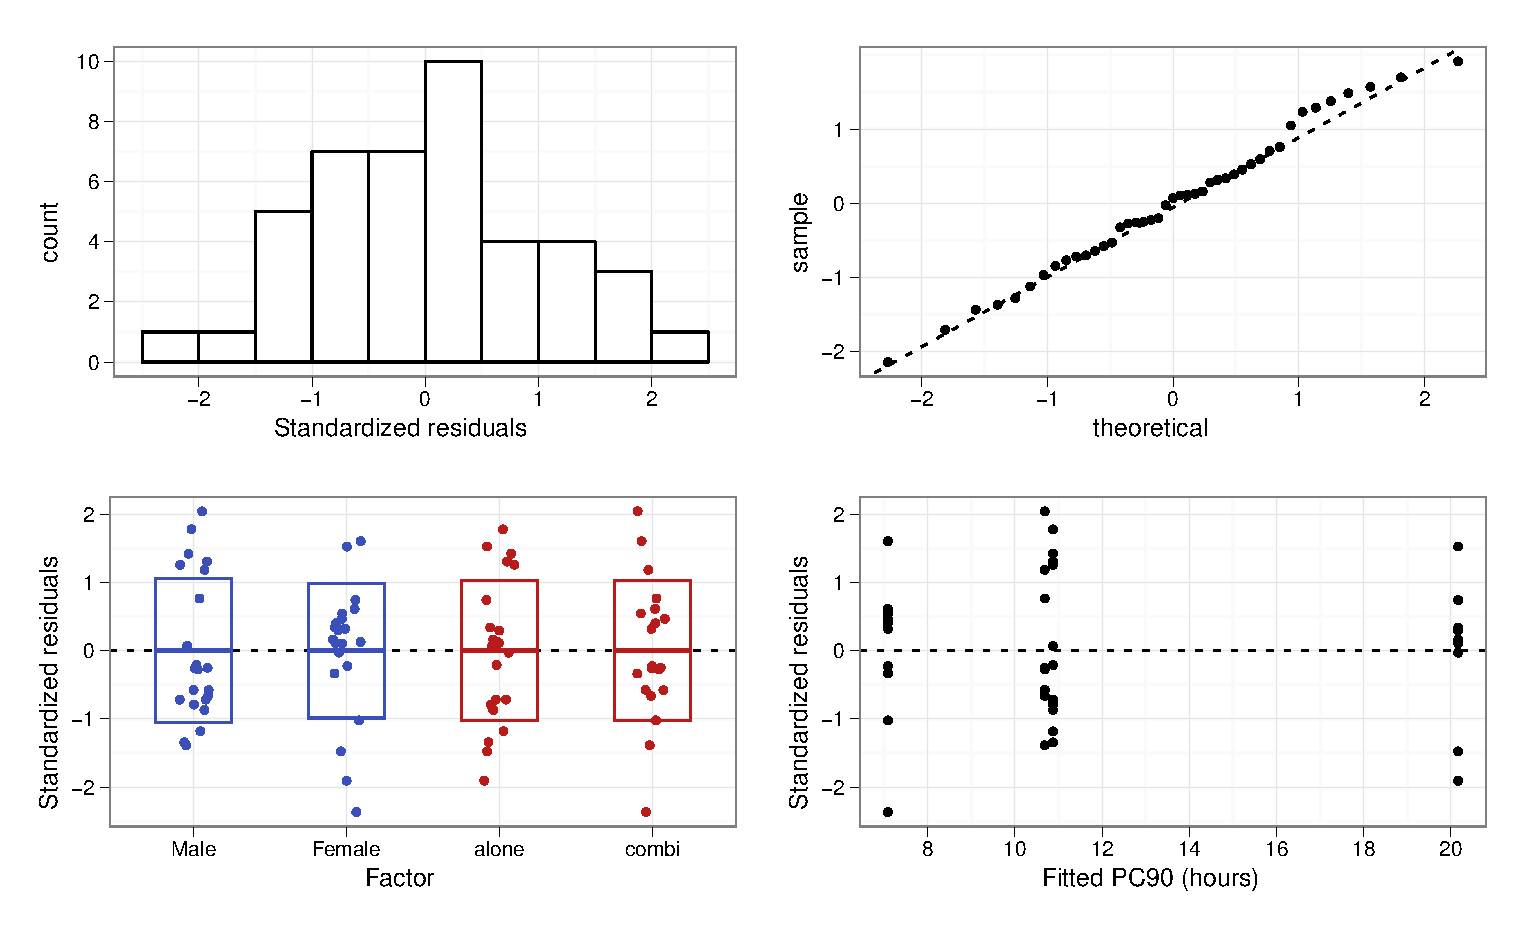
\includegraphics[width=150mm]{aov2rwt.eps} 
\caption{Residuals for the reduced model}
\label{aov2rwt}
\end{figure}

It can be seen that they are approximately normal and homoscedastic. The ANOVA table for this model is shown in Table \ref{aovreduced}, where the results are essentially the same as for the full model with some variation in the sex and treatment sums of squares due to the design matrix not being orthogonal.
%Sex            1  0.538   0.538  0.5939 0.44555  
%Treatment      1  5.152   5.152  5.6831 0.02209 *
%Sex:Treatment  1  5.166   5.166  5.6994 0.02191 *
%Residuals     39 35.353   0.906  
\begin{table}[h]
\centering
\caption{ANOVA table for the reduced model}\label{aovreduced}
\begin{tabular}{l|rrrrrl}
Source&Sum Sq.&df&Mean Sq.&$F$&P($>F$)\\
\hline
$Sex$				& 0.538 & 1 & 0.538 & 0.594 & 0.446 & \\
$Treatment$			& 5.15   & 1 & 5.15   & 5.68   & 0.022 & *\\
$Sex\times Treatment$	& 5.17   & 1 & 5.17   & 5.70   & 0.022 & *\\
$Residuals$			& 35.35 & 39 & 0.906 &&&\\
\hline
Total&46.21&42&&&
\end{tabular}\\
\hspace{20em}*$<0.05$
\end{table}

The fitted coefficients for the reduced model are shown in Table \ref{coefreduced}.
%                         Estimate Std. Error t value Pr(>|t|)    
%(Intercept)               3.29767    0.46257   7.129 1.43e-08 ***
%SexFemale                 1.19286    0.66887   1.783   0.0823 .  
%Treatmentcombi           -0.02899    0.52369  -0.055   0.9561    
%SexFemale:Treatmentcombi -1.79917    0.75363  -2.387   0.0219 *  
\begin{table}[h]
\centering
\caption{Fitted coefficients for the reduced model}\label{coefreduced}
\begin{tabular}{l|rrrc}
Factor levels&Coefficient&S.E.&$t$&P($>|t|$)\\
\hline
Male, single ($\mu$)			& 3.30 & 0.46 & 7.13 &  $1.4\times 10^{-8}$ \\
$\Delta$Female, single		& 1.19 & 0.67 & 1.78 & 0.082  \\
$\Delta$Male, combined 		& -0.029 & 0.52 & -0.055 & 0.96  \\
$\Delta$Female, combined	& -1.80 & 0.75 & -2.39 & 0.022  \\
\hline
\end{tabular}\\
Residual standard error: 0.95, Adjusted $R^{2}$: 0.18
\end{table}

With the corner-point constraint used only the male, single-treatment coefficient is absolute, with the other 3 being the relative change with change in factor level (indicated by $\Delta$). The $p$-values are perhaps a bit misleading in that the $p$-value for the mean $\mu$ corresponds to the null hypothesis $\mu=0$, with the other $p$-values corresponding to the hypotheses that the change in clearance time from the mean is 0 due to each change in factor level. Therefore, although only the female, combined treatment appears to be significantly different from the male, single treatment (-1.80), the mean difference between females on the single and combined treatments is larger i.e. $1.19-(-1.80)=2.99$. However, it is clear that there is no evidence to reject the hypothesis that the combined treatment gives the same mean clearance time as the single treatment for males.

Looking at inference for the clearance times will give a clearer picture of the relative effects of the factors.

\subsection{Inference for Clearance Times}
%\begin{itemize}
%\item The mean clearance time for male patients on the single treatment is $3.30^{2}=10.88$ hours with a 95\% confidence interval of ($2.54^{2},\ 4.05^{2})=(6.47,\ 16.41)$ hours.
%\item There is no evidence to reject the hypothesis that there is no difference between mean clearance times for male subjects on the single and combined treatments.
%\item Female subjects on the single treatment have a mean clearance time of $(3.30+1.19)^{2}=20.16$ hours with a 95\% confidence interval of (13.72, 27.85) hours.
%\item Female subjects on the combined treatment have a mean clearance time of $(3.30+1.19-0.029-1.80)^{2}=7.09$ hours with a 95\% confidence interval of (3.37, 12.16) hours.
%\end{itemize}
%$hours
%  fit lwr upr
%1  10   5  17
%2  20  12  29
%3  10   7  14
%4   7   4   9

%$minutes
%  fit lwr upr
%1  52  35  55
%2  10  21  54
%3  41  41  11
%4   5  41  59
Bearing in mind that a square-root transformation was used, we have from Table \ref{coefreduced}, the mean clearance times for each sex and treatment combination with 95\% confidence intervals shown in Table \ref{inference}.
\begin{table}[h]
\centering
\caption{Mean clearance times by sex and treatment}\label{inference}
\begin{tabular}{|l|c|c|}
\hline
&Clearance time PC90&95\% conf. int.\\
Factor levels&(hrs:mins)&(hrs:mins)\\
\hline
Male, single treatment 		& 10:52 & (5:35, 17:55) \\
Female, single treatment		& 20:10 & (12:21,  29:54) \\
Male, combined treatment	& 10:41 & (7:41, 14:11) \\
Female, combined treatment	& 7:05 & (4:41, 9:59) \\
\hline
\end{tabular}
\end{table}

It should be noted that these are confidence intervals for the estimate of the mean clearance time for the population. Prediction intervals for the expected clearance time of any one subject are considerably wider i.e. 95\% prediction intervals are: Male, single (0, 44) hours; Female, single (1, 62) hours; Male, combined (3, 24) hours; Female, combined (1, 19) hours.

The mean difference in the square root of PC90 between treatment groups, with confidence intervals and $p$-values calculated by Tukey's test for comparison of means \cite{montgomery} using the \texttt{TukeyHSD} \emph{R} function are shown below.
%                           diff   lwr   upr p adj
%Female:alone-Male:alone    1.19 -0.25  2.64  0.14
%Male:combi-Male:alone     -0.03 -1.51  1.45  1.00
%Female:combi-Male:alone   -0.64 -2.12  0.85  0.66
%Male:combi-Female:alone   -1.22 -2.73  0.29  0.15
%Female:combi-Female:alone -1.83 -3.34 -0.32  0.01
%Female:combi-Male:combi   -0.61 -2.15  0.94  0.72
\begin{table}[h]
\centering
%\caption{Difference in $\sqrt{\mathrm{PC}90}$ by Tukey's test}\label{tukey}
\begin{tabular}{l|ccrl}
&Diff.&95\% CI&$p$ adj.&\\
\hline
Male: combi - single 	& -0.03 & (-1.51, 1.45) & 1.00 &\\
Female: combi - single	& -1.83 & (-3.34,  -0.32) & 0.012 &*\\
\end{tabular}\\
*$<0.05$
\end{table}

It can be seen that there is evidence to reject the hypothesis of no difference between treatment groups for female subjects.

\newpage
Therefore, we can summarize the relative effects of the single and combined treatments:
\begin{description}
\item[Male subjects] - There is no evidence of a difference in mean clearance times between the two treatments for male subjects.
\item[Female subjects] - The mean clearance time for female subjects on the combined treatment is 13.1 hours shorter than for those on the single treatment with a 95\% confidence interval of (5.0, 22.7) hours.
\end{description}

The confidence intervals for the difference between groups in hours (i.e. the original scale before the square-root transformation used for the regression) are obtained by sampling 10,000 values from each of $[N(m_{a},s_{a}^{2})]^{2}$ and $[N(m_{b},s_{b}^{2})]^{2}$, where $a$ and $b$ specify the groups and $m$ and $s$ are the estimated mean and standard error of the groups. The percentiles of the distribution of the differences between these two samples are then taken.

\subsection{Comparison with other PC90 estimation methods}
The graphical investigation and model fitting procedure was repeated with the PC90 estimates obtained using the cubic polynomial and logistic regression techniques. The same overall trend and patterns of residuals were observed, leading to selection of the same optimal model (Equation \ref{reduced} on page \pageref{reduced}). The fitted coefficients are compared in Table \ref{compmeth}. 
\begin{table}[h]
\centering
\caption{Comparison of fitted models by 2 PC90 estimation methods}\label{compmeth}
\begin{tabular}{l|rr|rr|rr}
&\multicolumn{2}{c|}{log-linear}&\multicolumn{2}{c|}{cubic}&\multicolumn{2}{c}{logistic}\\
Factor levels&Coefficient&S.E.&Coefficient&S.E.&Coefficient&S.E.\\
\hline
Male, single ($\mu$)			& 3.30 & 0.46 & 3.43 &  0.49 & 4.06 & 0.52\\
$\Delta$Female, single		& 1.19 & 0.67 & 1.02 & 0.70  & 0.49 & 0.81\\
$\Delta$Male, combined		& -0.029 & 0.52 & -0.077 & 0.55 & -0.64 & 0.57\\
$\Delta$Female, combined	& -1.80 & 0.75 & -1.68 & 0.79  & -1.11 & 0.88\\
\hline
\end{tabular}
\end{table}

It can be seen that there is good agreement between the models fitted to the clearance times estimated by the log-linear and cubic methods. The estimated mean clearance times are compared in Table \ref{compinf}. Generally the same conclusions can be drawn regarding treatment effectiveness for the three methods, with the exception of male, single subjects with the logistic method. Remember that the logistic data has 8 subjects missing, all from the single treatment group, which most likely explains this discrepancy.
\begin{table}[h]
\centering
\caption{Mean clearance times by sex and treatment (hrs:mins)}\label{compinf}
\begin{tabular}{|l|cc|cc|cc|}
\hline
&\multicolumn{2}{c|}{log-linear}&\multicolumn{2}{c|}{cubic}&\multicolumn{2}{c|}{logistic}\\
Level		&Mean&95\% CI&Mean&95\% CI&Mean&95\% CI\\
\hline
M, single 		& 10:52 & (5:35, 17:55) &11:47& (6:00, 19:30) & 16:28 &(9:03, 26:05)\\
F, single		& 20:10 & (12:21,  29:54) &19:52&(11:46, 30:04) & 20:41&(10:38, 34:02)\\
M, combi	 	& 10:41 & (7:41, 14:11) &11:16&(8:02, 15:02) & 11:41 &(8:37, 15:13)\\
F, combi	 	& 7:05 & (4:41, 9:59) &7:16&(4:44, 10:21) & 7:49 & (5:21, 10:46)\\
\hline
\end{tabular}
\end{table}

\section{Dependence of clearance time on pre-dose parasite count}
\subsubsection*{Pre-dose count}\label{sec:predoseancova}
We might expect that subjects with a higher pre-dose parasite count would have a longer clearance time. To investigate this, the PC90 clearance time is plotted against pre-dose parasite count in Figure \ref{predose-ancova}. There is no obvious trend in clearance time with pre-dose parasite, nor when the data is split by centre, sex and treatment. Statistical tests such as Spearman's rho and ANCOVA (adding pre-dose count as a covariate to the ANOVA model) do not give any evidence of correlation of clearance time with pre-dose parasite count.
\begin{figure}[p]
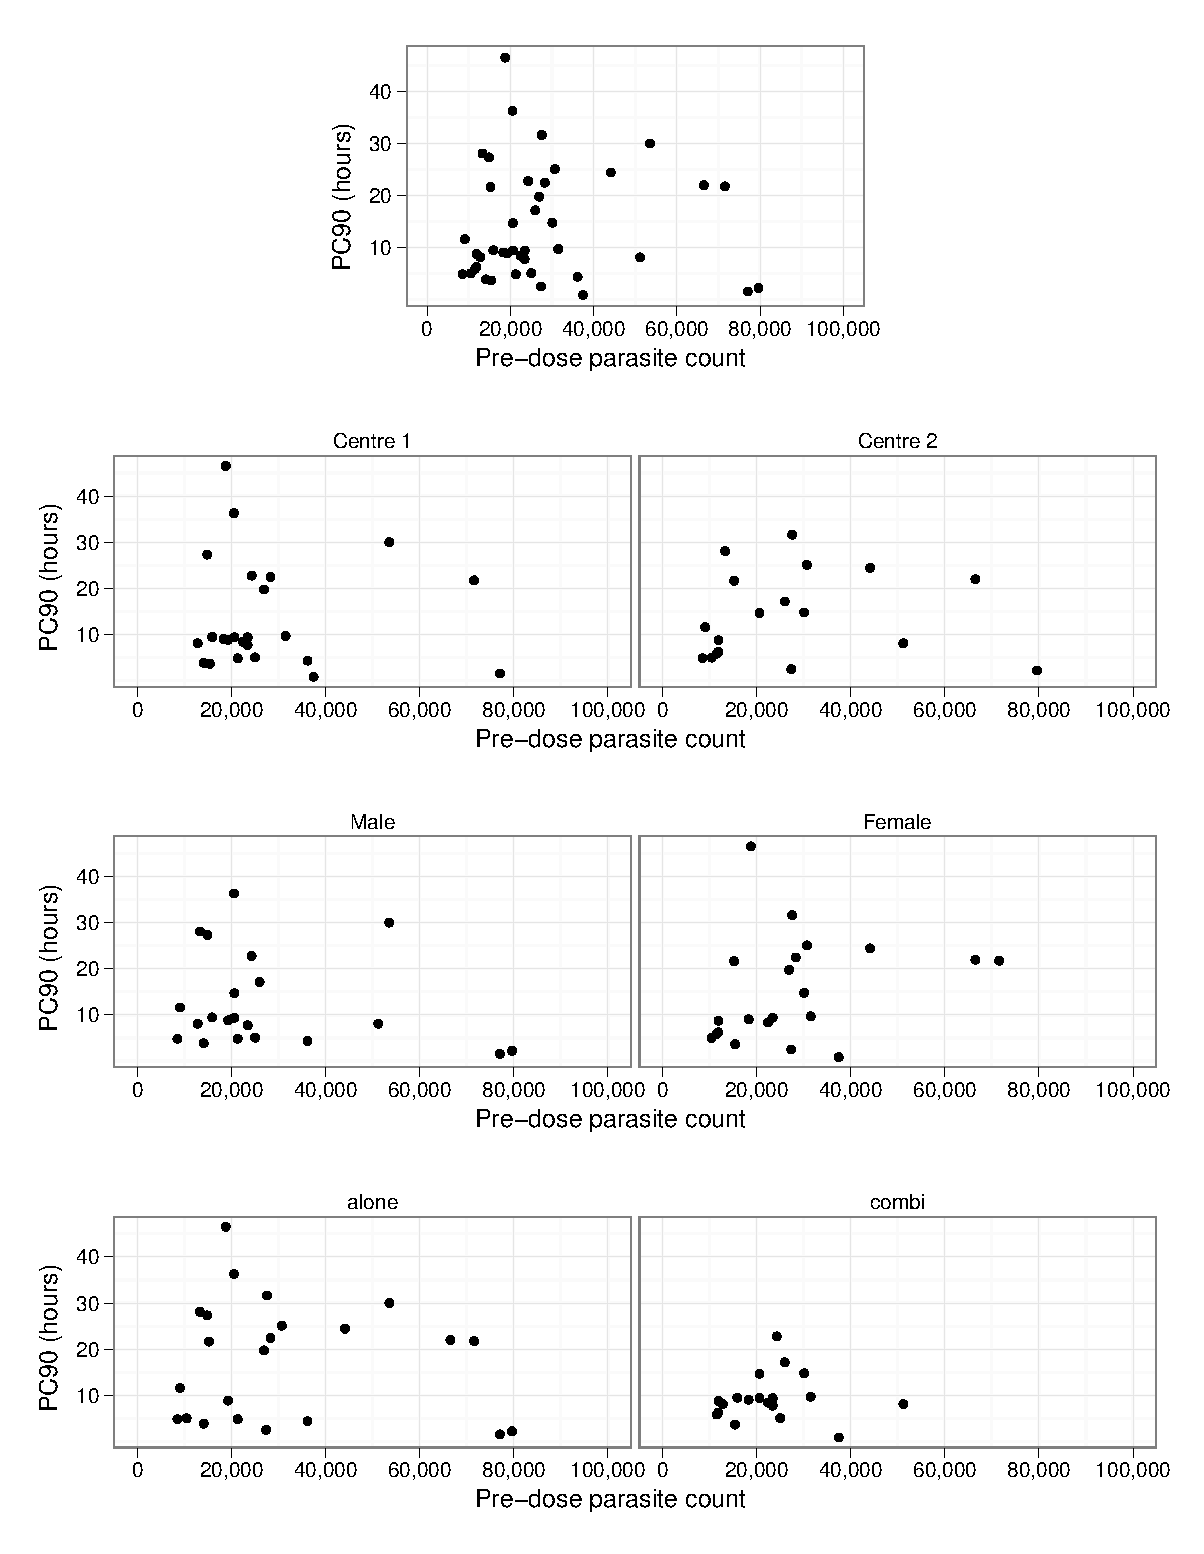
\includegraphics[width=150mm]{predose-ancova.eps} 
\caption{Dependence of clearance time on pre-dose parasite count}
\label{predose-ancova}
\end{figure}

%The fitted ANCOVA model is a modification of the reduced ANOVA model \ref{reduced} on page \pageref{reduced} adding the pre-dose parasite count as a covariate with all interactions with sex and treatment. This ANCOVA model is compared to the ANOVA model in Figure \ref{compancova}. It can be seen that the ANCOVA model isn't a significant improvement.

\subsubsection*{Time of pre-dose count}\label{sec:pretimeancova}
The clearance time is plotted against the time before first dose at which the pre-dose count was recorded in Figure \ref{pretime-ancova}. Although it looks like there is some positive correlation between the time of pre-dose recording and clearance times, statistical tests reveal no evidence to reject the hypothesis that the effect of pre-dose recording time is negligible. It could be that we do not have enough power with this sample to detect an effect if there is one. 
\begin{figure}[p]
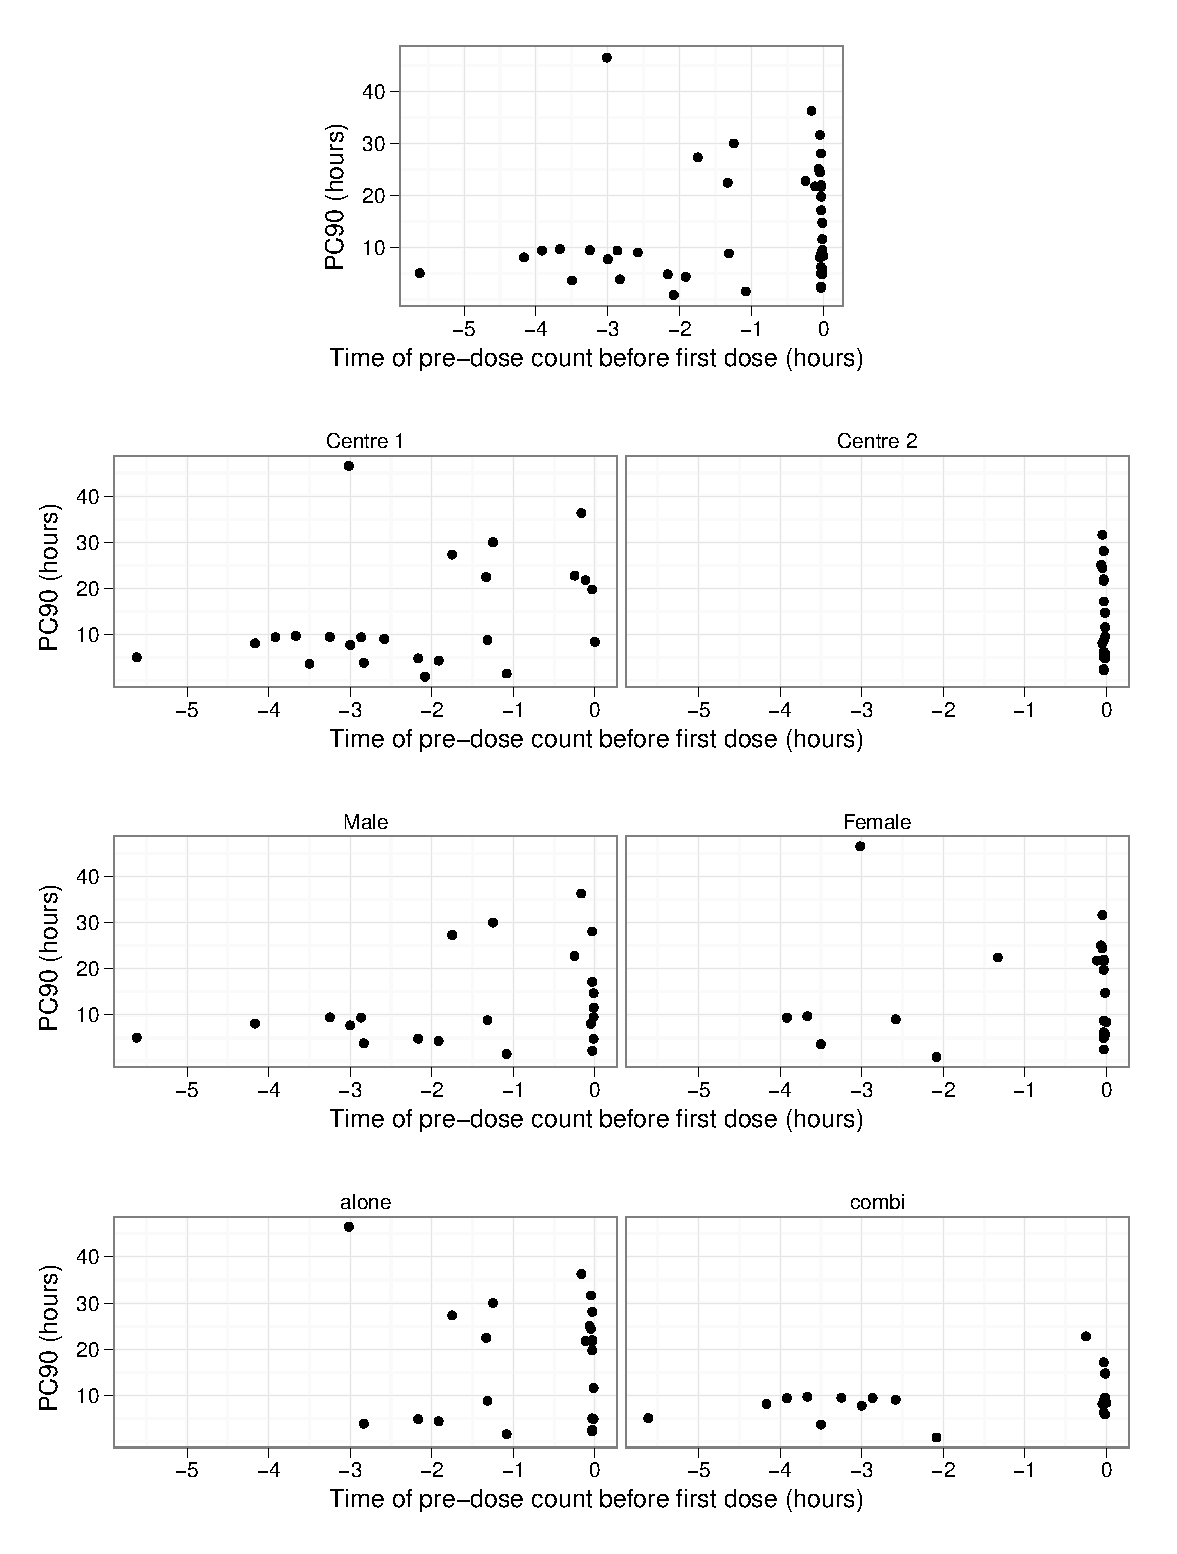
\includegraphics[width=150mm]{pretime-ancova.eps} 
\caption{Dependence of clearance time on the time before first dose that the pre-dose parasite count was recorded}
\label{pretime-ancova}
\end{figure}

%The ANCOVA model with time of pre-dose count as a covariate is compared to the ANOVA model in Figure \ref{compancova2}.
%It looks like there is a significant interaction with time of pre-dose count for female subjects, but this is mainly attributed to a single high-leverage datum and the coefficient in the ANCOVA model isn't highly significant ($p$=0.077). It could be that we simply don't have high enough power in this experiment to detect this interaction.

%\begin{figure}[p]
%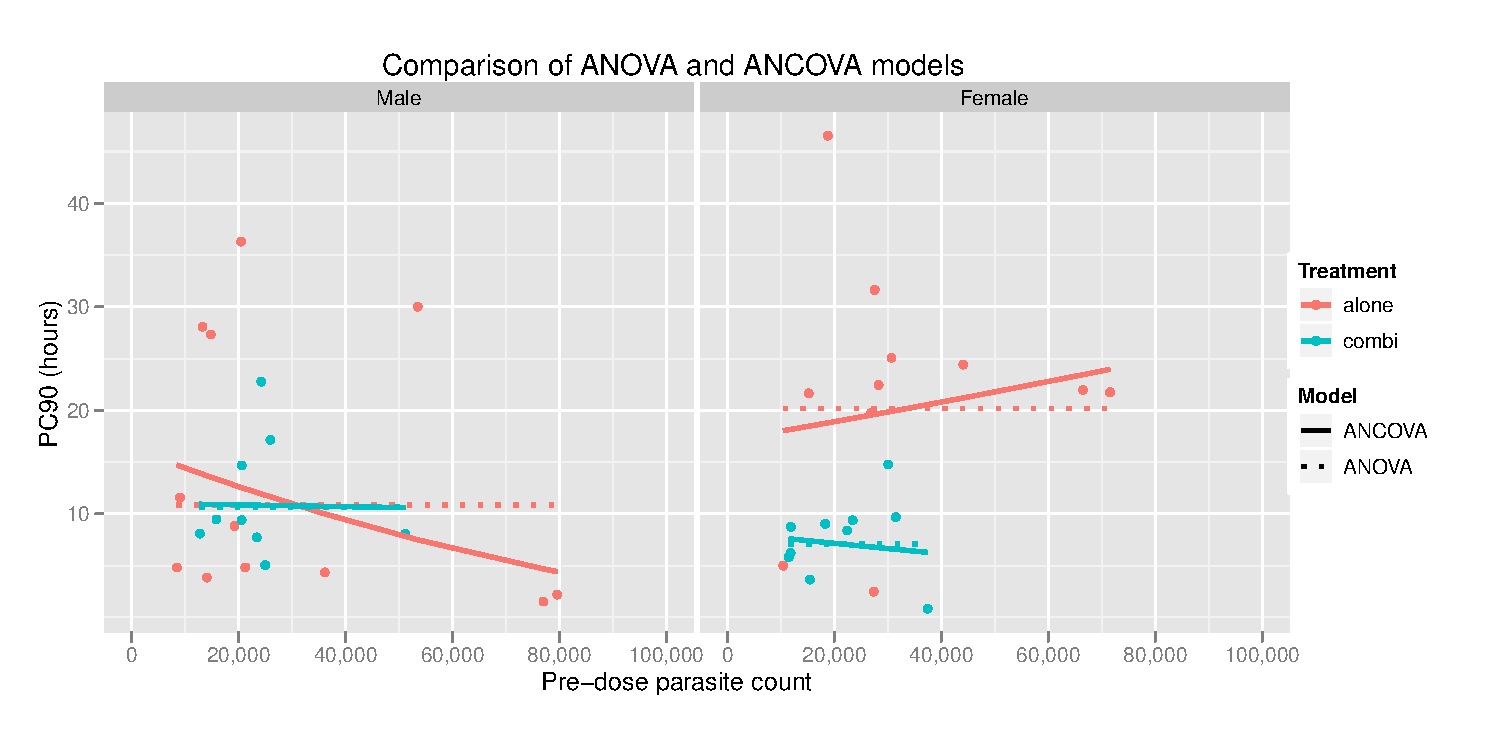
\includegraphics[width=150mm]{compancova.eps} 
%\caption{Comparison of ANOVA and ANCOVA models}
%\label{compancova}
%\end{figure}
%\begin{figure}[p]
%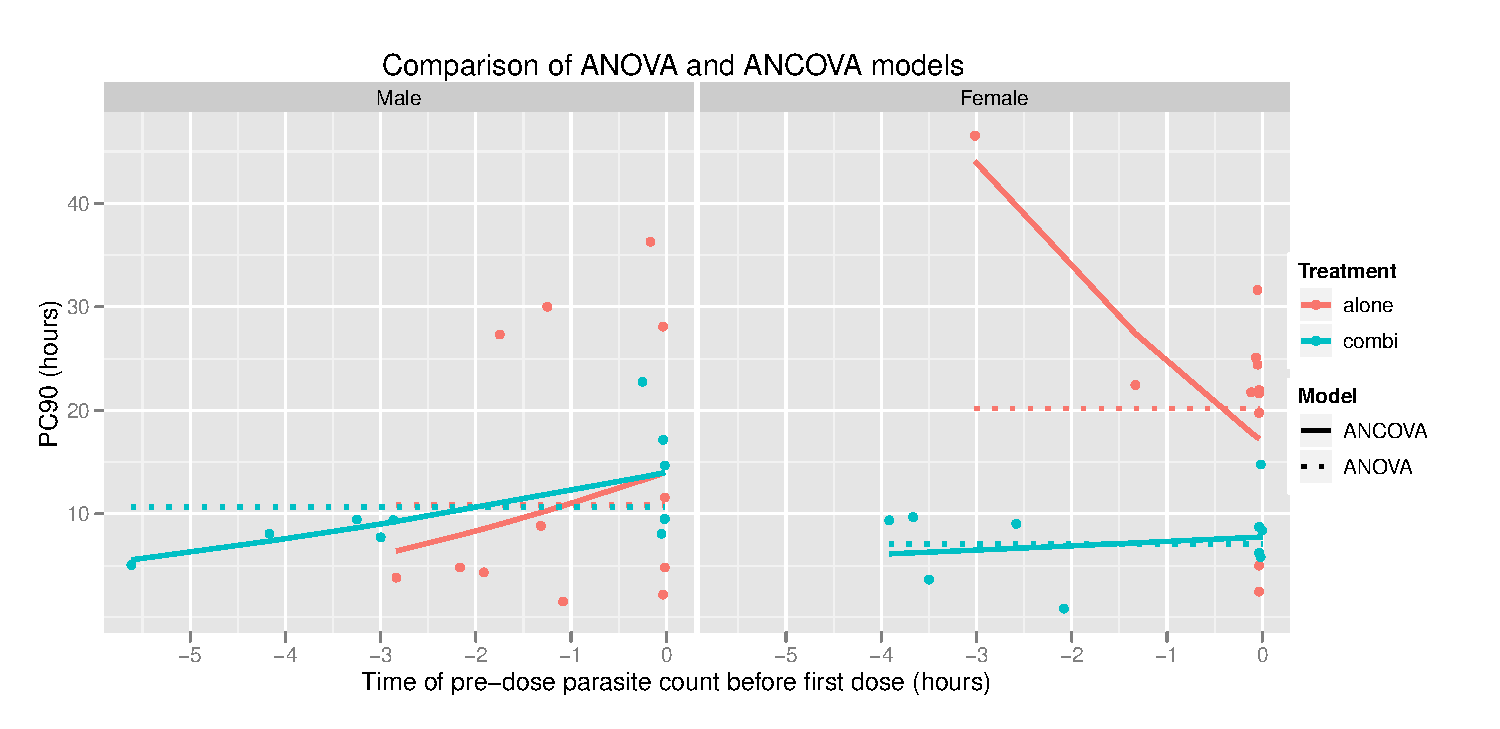
\includegraphics[width=150mm]{compancova2.eps} 
%\caption{Comparison of ANOVA and ANCOVA models}
%\label{compancova2}
%\end{figure}
\clearpage
\section{Non-parametric methods}
As an additional verification of the analysis so far based on parametric methods, we can compare the results with analysis of clearance times using non-paramteric, distribution-free methods.

\subsection{Non-parametric statistics}
\subsubsection*{ANOVA using ranks}
One non-paramteric alternative to two-way ANOVA is to calculate the $F$ statistics using the ranks of the data instead of the actual values of the dependent variable \cite{conover}. The results of ANOVA using ranks are shown in Table \ref{aovranks} with the $p$-values from the parametric analysis (Table \ref{aovreduced} on page \pageref{aovreduced}) shown for comparison.
%> summary(PC90.loglinr.rank.aov)
%              Df Sum Sq Mean Sq F value  Pr(>F)  
%Sex            1   78.3    78.3  0.5562 0.46025  
%Treatment      1  390.6   390.6  2.7758 0.10371  
%Sex:Treatment  1  664.9   664.9  4.7247 0.03587 *
%Residuals     39 5488.2   140.7    
\begin{table}[h]
\centering
\caption{ANOVA using ranks}\label{aovranks}
\begin{tabular}{l|rrrrrl|rl}
Source&Sum Sq.&df&Mean Sq.&$F$&P($>F$)&&P$^{\dag}$($>F$)\\
\hline
$Sex$				& 78.3 & 1 & 78.3 & 0.556 &  0.460 && 0.446& \\
$Treatment$			& 390.6   & 1 & 390.6   & 2.78 & 0.104&  & 0.022&* \\
$Sex\times Treatment$	& 664.9   & 1 & 664.9   & 4.72 & 0.036&*   & 0.022&* \\
$Residuals$			& 5488.2 & 39 & 140.7 &&&&\\
\hline
Total&6622&42&&&&
\end{tabular}\\
P$^{\dag}$: $p$-value from parametric analysis\qquad*$<0.05$
\end{table}

It can be seen that the non-parametric method shows a significant interaction effect at the 5\% level, but not for the main treatment effect unlike the parametric analysis. It could be that there is only an effect of treatment for one sex (Figure \ref{pc90interaction} on page \pageref{pc90interaction} would suggest this), although Toothaker \textit{et al.} \cite{toothaker} note that these tests should not be used to test for main effects in the presence of an interaction and vice-versa.

\subsection{Resampling methods}\label{section:resampling}
Another alternative to parametric ANOVA is to resample the data using either the permutation or bootstrap methods and thereby determine the sampling distribution of our statistics \cite{manly}. There are several different approaches for resampling ANOVA models with crossed factors, such as ours, by permutation \cite{manly, anderson}. Three of them are:
\begin{description}
\item[Unrestricted permutation of raw data] - The raw data is randomized between all groups and the $F$ statistics recalculated for each randomization. Anderson and Braak note that this is an approximate test for both main effects and interactions \cite{anderson}.
\item[Permutation of residuals] - An approximate test for an interaction effect by controlling for main effects can be performed by defining residuals
$$r_{ijk}=y_{ijk}-\bar{y}_{i..}-\bar{y}_{.j.}+\bar{y}_{...}$$
where $\bar{y}_{i..}$ is the mean response at level $i$ of the first factor, $\bar{y}_{.j.}$ the mean response at level $j$ of the second factor and $\bar{y}_{...}$ the overall mean. The $F$ statistics are then calculated from ANOVA using these residuals as the response.
\item[Restricted permutation of raw data] - To test for a main effect the response can be randomized \emph{between} levels of the main effect but \emph{within} the levels of the other factors. For example, to test for a treatment main effect with our data, we would randomize the treatment of each observation but keep the sex and centre static. Only the $F$ statistic of the main effect being randomized is relevant in the ANOVA output from this method. Anderson and Braak note that this is an exact test for main effects, but is only reasonable if there is no evidence of an interaction effect \cite{anderson}.
\end{description}
Manly finds by simulation that the $F$ statistic gives the most consistent results across all three methods, as opposed to using mean square residuals for example \cite{manly}. Anderson and Braak note that permutation of residuals is significantly more powerful that permutation of raw data when errors are highly non-normal, for example lognormal \cite{anderson}.

These 3 permutation methods were implemented in \emph{R}\footnote{The code is listed in Appendix \ref{R:resamp} on page \pageref{R:resamp}.}. The results for the full 3-way ANOVA model are shown in Table \ref{aovresamp} compared to the parametric $F$ test for the square-root transformed model fitted by weighted least-squares.
\begin{table}[h]
\centering
\caption{$p$-values for 3-way ANOVA $F$ statistic determined by resampling.\\Values not relevant to test in \small{\textit{small italics}}.}\label{aovresamp}
\begin{tabular}{l|rrrr|r}                   
Source						&P($>F_{1}$)&P($>F_{2}$)&P($>F_{3t}$)&P($>F_{3s}$)&P$^{\dag}$($>F$)\\
\hline
$Centre$     					& 0.971 & \small{\textit{0.720}} & \small{\textit{0.008}} & \small{\textit{0.173}} & 0.354 \\    
$Sex$        					& 0.370 & \small{\textit{0.912}} & \small{\textit{0.008}} & 0.364 & 0.420 \\  
$Treatment$  					& 0.009 & \small{\textit{0.962}} & 0.007 			   & \small{\textit{0.126}} & 0.029 \\
$Centre\times Sex$ 				& 0.781 & 0.780 			& \small{\textit{0.174}} & \small{\textit{0.774}} & 0.956 \\
$Centre\times Treatment$ 		& 0.361 & 0.352 			& \small{\textit{0.334}} & \small{\textit{0.113}} & 0.462 \\
$Sex\times Treatment$     		& 0.026 & 0.027 			& \small{\textit{0.027}} & \small{\textit{0.029}} & 0.017 \\
$Centre\times Sex\times Treatment$& 0.634 & 0.637 			& \small{\textit{0.629}} & \small{\textit{0.607}} & 0.596
\end{tabular}\\
$F_{1}$ - Unrestricted permutation; $F_{2}$ - Permutation of residuals; $F_{3t}$ - Permutation restricted to treatment; $F_{3s}$ - Permutation restricted to sex; P$^{\dag}$ - Parametric result\\
10,000 samples for each method
\end{table}

It can be seen that the $p$-values obtained by resampling lead to the same conclusions as the parametric test. In particular that there is no evidence to reject the hypothesis that the effect of centre is negligible. Accordingly, the results for the reduced 2-way model are shown in Table \ref{aovresampr}.
\begin{table}[h]
\centering
\caption{$p$-values for 2-way ANOVA $F$ statistic determined by resampling.}\label{aovresampr}
\begin{tabular}{l|rrrr|r}                   
Source						&P($>F_{1}$)&P($>F_{2}$)&P($>F_{3t}$)&P($>F_{3s}$)&P$^{\dag}$($>F$)\\
\hline
$Sex$        					& 0.375 & \small{\textit{0.951}} & \small{\textit{0.004}} & 0.360 & 0.446 \\  
$Treatment$  					& 0.007 & \small{\textit{0.981}} & 0.007 			   & \small{\textit{0.086}} & 0.022 \\
$Sex\times Treatment$     		& 0.049 & 0.049 			& \small{\textit{0.049}} & \small{\textit{0.041}} & 0.022 \\
\end{tabular}\\
10,000 samples for each method
\end{table}
It can be seen that the hypothesis tests for main effects and interactions produce the same results at the 5\% level for all the permutation techniques and the parametric model. For the permutation  methods the interaction effect is only just significant at the 5\% level. Anderson and Braak \cite{anderson} note that the parametric $F$ test is more powerful than permutation techniques when the residuals are approximately normal, as they are for our square-root transformed model fitted by weighted least-squares (Figure \ref{aov2rwt} on page \pageref{aov2rwt}).

\subsubsection*{Non-parametric confidence intervals}
Our parametric 2-way ANOVA identified that there is only a significant difference between the clearance times of the two treatments for female patients and we derived confidence intervals for the reduction in clearance time for female patients using the combined drug treatment (page \pageref{compinf}).

We can derive a non-parametric confidence interval for the improvement in clearance time for female patients using the combined treatment by resampling. If we select only female subjects and permute the clearance times between treatments then we can derive a sampling distribution of the difference between means under the null hypothesis
$$H_{0}:\mu_{s}-\mu_{c}=0$$
i.e. the mean clearance time for the single treatment $\mu_{s}$ is the same as that for the combined treatment $\mu_{c}$. To test the hypothesis that the difference between the treatments is $k$ we use the null hypothesis
$$H_{0}:\mu_{s}-\mu_{c}-k=0$$
and accordingly subtract $k$ from the clearance times for the single treatment before permuting the values. Now 95\% confidence intervals for the difference between treatments are equal to the minimum and maximum values of $k$ that are not rejected by our test at the 5\% level. Therefore, the algorithm to find the confidence interval is:
\begin{enumerate}
\item Choose a value of $k$ that we think is at the 95\% confidence limit for the difference between clearance times. Good initial choice are the limits from the parametric test.
\item Subtract $k$ from the original clearance times for the single treatment.\label{start}
\item Calculate the statistic $T_{obs}=\mu_{s}-\mu_{c}$.\label{fstat}
\item Permute the clearance times between treatments $N-1$ times and at each permutation calculate $T^{*}_{i}=\mu_{s}^{*}-\mu_{c}^{*}$.
\item Calculate the $p$-value of our $T_{obs}$ statistic from step \ref{fstat} by its percentile in the set of $N$ values comprised of $T_{obs}$ and $T_{i=1,...,N-1}^{*}$ from the $N-1$ permutations.
\item If the $p$-value is $<0.05$ and we are looking for the lower limit of the 95\% confidence interval or $p>0.05$ and we are looking for the upper limit, increase $k$ and go to step \ref{start}. If $p>0.05$ and we are looking for the lower limit or $P<0.05$ and we are looking for the upper limit, decrease $k$ and go to step \ref{start}.
\item At $p\approx 0.05$ we have estimates of our 95\% confidence limits.
\end{enumerate}
This algorithm was implemented in \emph{R}, giving a 95\% confidence interval for the improvement in mean clearance time of the combined treatment over the single treatment for female subjects of (6.5, 22.5) hours, corresponding to $p$-values of 0.0510 and 0.0496 respectively, achieved by repeated samples of 10,000. This gives reasonable agreement with the interval of (5.0, 22.7) hours obtained by the parametric ANOVA method.

\section{Key results}
The log-linear method was identified in chapter \ref{ch:derivation} as the most suitable estimate of PC90, the time for 90\% of parasites present before treatment to be cleared from the blood. Accordingly, these PC90 values, one for each of the 43 subjects were analysed, primarily for their dependence on experimental factors centre, sex and treatment. The key findings of this analysis were:
\begin{itemize}
\item Initial graphical analysis indicates no dependence of PC90 on centre, but that female subjects on the combined treatment have a mean PC90 some 10-15 hours shorter than those on the single treatment. There is no obvious difference between male subjects on the single and combined treatments.
\item The variance of PC90 for subjects on the single treatment seems larger than for those on the combined treatment.
\item Analysis of residuals from 3-way ANOVA of PC90 by centre, sex and treatment indicates that a square root transformation of PC90 is required to stabilise the variance of the residuals with magnitude of PC90.
\item Fitting by weighted least-squares is required to stabilise the variance of the ANOVA residuals between treatment groups. Accordingly, the least-squares fitting is weighted by the variance within the two treatment groups. 
\item 3-way ANOVA by centre, sex and treatment, after the appropriate variance stabilising measures gives no evidence to reject the hypothesis that centre has no effect on PC90.
\item 2-way ANOVA by sex and treatment shows good evidence to reject the hypothesis that treatment has no effect on PC90 and the hypothesis that there is no interaction of sex and treatment that effects PC90 ($P<0.05$ for both).
\item There is no evidence to reject the hypothesis that there is no difference in mean PC90 clearance times between treatments for male subjects.
\item There is good evidence ($P<0.05$) to reject the hypothesis that there is no difference in PC90 clearance times between treatments for female subjects. The mean difference is 13.1 hours shorter for the combined treatment with a 95\% confidence interval of (5.0, 22.7) hours.
\item PC90 estimates using the cubic polynomial regression method lead to the same conclusions regarding treatment effect as the log-linear interpolated estimates. The logistic regression estimates are generally compatible with observed discrepancies most likely due to missing data for the logistic method.
\item There is no evidence to reject the hypotheses that the PC90 clearance time is independent of the pre-dose parasite count and independent of the time at which the pre-dose count was taken.
\item Non-parametric methods support the findings of the parametric analysis in that only the difference between treatments for female subjects is significant. An appropriate resampling method estimates a 95\% confidence interval for the decrease in PC90 clearance time for female subjects on the combined treatment of (6.5, 22.5) hours.
\end{itemize}